\graphicspath{{2_Body/Figures/}}




\chapter{Methodologie}
\label{chapter:body}
\thispagestyle{myheadings}




\chapter{Theoretisch kader}
\subsection{MODE CONFUSION }
Mode confusion tredd op als gepbserveerd gedrag van een technisch systeem niet past in het gedragspatroon dat de gebruiker in zijn beeldvorming heeft  en ook niet met voorstellingsvermogen kan bevatten.
\subsection{Wat is automatiseringsparadox}
Gemak dient de mens. Als er veel energie wordt gestoken in de ontwikkeling van hulmiddelen die taken van werknemers overemen heeft dat tot resultaat dat veel productieprocessen worden geautomatiseerd. De vraag is dan of vanuit mechnisch wereldpunt de robot niet de rol van de mens overneemt en of de mens nog de kwaliteiten heeft om het werk zelf te doen.

\url{https://www.dalton.nl/literatuur/item/252-de-automatiseringsparadox}
\url{https://www.debicker.eu/de-automatiseringsparadox/}
\url{https://vse.nl/de-paradox-van-de-industriele-automatisering/}
\url{https://automatie-pma.com/nieuws/industriele-automatiseringsparadox}
\url{https://blog.xot.nl/2016/11/21/slimme-apparaten-maken-ons-dom-en-kwetsbaar/index.html}

\subsection{Wat is een model}
\subsubsection{Conceptueel model}
Om duding te geven aan het grote plaatsje
\subsubsection{in vivo model}
Levende organismendie in de werkelijkheid of in een laboriatrum vergelijkbare eigenschappen bezitten als bestaande fenomenen in de werkeljkheid. Deze objecten zijn vergelijkbaar met werkelijkobjecten en geven vergelijkbare resultaten
\subsubsection{in vitro model}
Een model dat dezelfde condities biedt  buiten het onderzoeksobject om, maar is voldoende vergelijkbaar om vergelijkbare processen te simuleren.
Zowel invivo als in vitro modellen zijn beperkt door de materialen die beschikbaar ijn voor onderzoek en de arbeidsomstandigheden waaronder ze worden gebruikt. Desondanks zijn het geen werkelijke natuurlijke modellen dus vvoor een onderzoek kan boedt het geen volledige uitsluitsel.
\subsubsection{In silicio model}
Ee veelzijdig object. Het verwijst naar simulaties die gebruik maken van wiskundige modellen in computer,een zijn dus afhankelijk van silicone chips. In silico model analyseert  wiskundige vergelijkingen om resultaten te geven onder bepaalde omstandigheden. Deze vergelijkingen vertellen iets over de correlatie van verschillende objecten van een wetenschappelijk onderzoek. OM deze modellen te kunnen gebruiken is het noodzakelijk te omschrijven waat de fenomenen in kwestie van onderzoek zijn door middel van getallen. Kwanttitatieve relaties kunnen worden geintegreerd in het model en waar deze relaties complex zijn is een computer noodzakelijk deze op telossen. Vaak worden hierbij verschillende mechanismen gebruikt. Als je bijvoorbeeld de prijsontwikkeling van een marsreep in kaart wilt brengen.
\subsubsection{in simulacra model}

\subsection{World and machine samenvatting}
Waarom zijn wij engineers? Omdat we bruikbare apparaten willen laten functioneren in de wereld waarin we leven. Dat doen we door de machine te beschrijven en deze beschrijving van instructies bieden we aan onze computer opdat deze als de attribuut en gedragingen uitleest zoals wij die hebben omschreven. Dit alles op basis van theoretische funderingen en praktisch inzicht. 

Het doel van een machine is om te worden geinstalleerd en te worden gebruikt. De eisen die we stellen zitten in de omgeving en in de wereld en de machine is slechts de oplossing die we bedenken om aan een eis te voldoen. 

De relatie machine-wereld world gecategoriseerd in: 

Het modelleer aspect: waar een machine de wereld simuleert 

Het interface aspect: waar er fysieke interactie is tussen de machine en de wereld 

Het engineering aspect: waar de machine zich gedraagt als een controlemotor gebruikmakend van de gedragingen van de omgeving in de wereld 

Het probleem aspect: waar de omgeving in de wereld en de omvang van het probleem invloed heeft op de machine en de oplossing 

Het modelleer  of simulatie aspect over een deel van de wereld. Er zijn data,object en proces modellen. Het doel van een model is toegang te geven tot informatie over die wereld. Door het opvangen van statische weergaven en gebeurtenissen kunnen wij deze gebruiken van opgeslagen informatie die we kunnen hergebruiken. Een model kan bruikbare informatie bevatten omdat zowel het model als de wereld warin het model zich bevind gemeenschappelijke omschrijvingen hebben die waar zijn voor zwel het model als voor de wereld. Daarbij moet gesteld worden dat de interpretatie van een model verschilt met een interpretatie van de wereld. 

Omdat zowel de wereld als de machine fysieke realiteiten zijn an niet slechts abstracties, zijn de gemeenschappelijke beschrijvingen slechts een deel van de werkelijheid van beide objecten. For elk object zijn er meerdere beschrijvingen. Toch maken niet alle omschrijvingen deel uit van het getoonde reportoire. Zoals niet alle eigenschappen van een boek; meer dan een auteur, pseudoniemen, een onderdeel van een reeks, een gerevisiteerde versie, worden gereflecteerd in een database.  

Het interface aspect. Een machine kan een probleem in de wereld oplossen als de wereld en de machine phenomena kunnen uitwisselen. Maar de participatie is niet symmetrisch: een status kan als phenomena worden uitgewisseld maar slechts een partij kan er invloed op uitoefenen maar beiden kunnen dezelfde status signaleren. 

Het engineering aspect gaat over requirements, specificaties, en programma’s. Requirements hebben betrekking op phenomena in de wereld. Een programma heeft alleen betrekking tot de machinale phenomena. Het doel van programma’s is om eigenschappen en gedragingen te omschrijven van de machine ten behoeve van de gebruiker. Tussen de requirements en de programma’s zitten de specificaties. Omdat programma’s dan wel beschrijvingen zijn van een gewenste machine, maar dat moeten beschrijvingen zijn van de  machines  die de computers kunnen uitvoeren zodanig dat de computer deze beschrijvingen ook zo kan interpreteren. De engineer moet  de eigenschappen van de wereld kennen en begrijpen en deze eigenschappen manipuleren en laten werken met als doel het dienen van het systeem. 

Het probleem aspect. Het onderscheid tussen specificatie en implementatie. Het probleem zit in de relatie van de machine en de wereld. De machine brengt de oplossing maar het probleem zit in de wereld. Een vertoog over een probleem moet dus gaan over de wereld en over de opvatting die de gebruiker heeft in de wereld. Omdat de wereld veelzijdig is moeten we ervan uit gaan dat er verschillende soorten problemen zijn. Een realistisch probleem wordt dus niet opgelost met een simpele hiërarchische structurele aanpak en een homogene decompositie maar met een paralleele structurele oplossing waar beide kanten van het probleem worden opgelost. 



Ontkenningen 

We hebben als engineers de taak om een machine te bouwen aan de hand van de specificaties opgeleverd door de opdrachtgever. Een engineer heeft niet als taak de fitheid voor een doeleind te onderzoeken, maar wel de haalbaarheid naar een doeleind aan de hand van kennis, tijd, resources, budget en ontwikkelmethodiek. Daaruit komt naar voren dat een engineer zich richt op: elicitation (schetsen van een requirement), description (omschrijving) en analyse van de requirements waaraan het systeem moet voldoen. Vertaalt naar de volgende vragen: Wat is precies de klantwens?  Wat is de precieze omschrijving van het probleem? Voor welke doelen wordt het systeem gebouwd? Welke functies moet het systeem hebben? 

Denial by hacking: obsessief bezig zijn met een systeem omdat het de gebruiker veel macht geeft. Een uitgebreidheid van een systeem zorgt er soms voor dat mensen niet meer geprikkeld zijn na te denken over probleemstellingen, domein beschrijvingen en analyse. 

Denial by a abstraction. Wiskundige benaderingen van werkelijke problemen is  een belangrijke intellectuele strategie om problemen te formuleren. Een software ontwikkelaar moet een probleem kunnen omschrijven in zo min mogelijk woorden, maar de complexiteit ligt in de oplossing. 

Denial by vagueness. De vaagheid van een omschrijving is terug te vinden in: 

Von Neumann’s principe 

Principe van reductionisme 

Shanley principe 

Montaingnes’s principe 

Von Neumand principe 

Voor een vocabulair  moet een grondslag zijn ontwikkeld waarmee gesproken kan worden over de wereld en de machine. Belangrijke phenomenen moeten geindtifieerd worden, door middel van een grondregel  of ‘herkenningsregel’ moet een fenomeen worden herkend, en vervolgens het fenomeen een formele term geven die gebruikt wordt als duiding van een bepaalde omschrijving. Dan moet voor de formele term een symbool gevonden worden. Samen vormen de grondregel en het symbool een designatie. 

Principe van reductionisme 

Simpelweg het openbreken van termen met een weerlegbare definitie totdat alle begrippen die worden gebruikt om iets te duiden  niet meer te herconstrueren zijn in hun definitie. 

Shanley principe 

Er bestaan volgens dit principe geen scherpe verdelingen in de wereld zoals wetenschappers soms denken. Een strenge opvatting over de wereld waarin een individu geclassificeerd kan worden als een onsamenhangend geheel. Maar dat is slechts een opname van een beeld. De werkelijkheid staat soms toe dat een elementair individueel object in verschillende classificaties verschillende getypeerd kan worden in een andere setting of view. 

Montaignes principe 

De incative mood; gaat over wat we beweren waar te zijn. 

De optitative mood; gaat over wat we willen dat waar is 
\subsection{SIX Variable model}
Optitatieve statements omschrijven de omgeving zoals we het willen zien vanwege de machine. 

Indicatieve statements omschrijven de omgeving zoals deze is los van de machine. 

Een requirement is een optitatief statement omdat ten doel heeft om de klantwens uit te drukken in een softwareontwikkel project. 

Domein kennis bestaut uit indicatieve uitspraken die vanuit het oogpunt van software ontwikkeling relevant zijn. 

Een specificatie is een optitatief statement met als doel direct implementeerbaar te zijn en ter verondersteuning van het natreven vande requirements. 

Drie verschillende type domeinkennis: domein eigenschappen, domein hypothesen, en verwachtingen. 

Domein eingenschappen  zijn beschrijvende statementsover een omgeving en zijn feiten.Domein hypotheses  zijn ook beschrijvende uitspraken over een omgeving, maar zijn aannames. 

Verwachtingen zijn ook aannames, maar dat zijn voorschrijvende uitspraken die behaald worden door actoren als personen, sensoren en actuators. 

Het verschil tussen essentie en incarnatie van een systeem. Een essentie bevestigd de  mogelijkheden dat een systeem moet hebben om te voldoen aan de eise, ongeacht hoe het systeem is geimlementeerd. De incarnatie bevestigd of omvat de mogelijjkheden die te maken hebben met details omtrent implementatie. Een heuristiek voor het identificeren van de essentie van een systeem is de aanname van perfecte technologie, ofwel de aanname dat de technologie binnen een systeem perfect is. Om essentie te indentificeren nemen we aan dat technologie buiten de machine om perfect is. Zouden we incarnatie overwegen dan wordt de aanname van perfecte machin-externe technologie opgeheven. 

Voor de documentatie van contextuele beslissingen en opties/alternatieven wordt de OVM (Orthogonale variability Model) gebruikt. Oorspronkelik was deze methode bedoeld om de variatiepunten en de variant van een productlijn samen met hun variabele afhankelijkheden( mandatory, optional, alternative)  en beperkende afhankelijkheden(requires en excludes)te omvatten. De variant kan worden gerelateerd aan een ontwikkelartefact zoals een requirement of een diagram als een zogenoemde artefact dependency. Een artefact is dan gedefinieerd als variabele. Voor de documentatie van de keuzen die we maken is een selectie model gemaakt. We gebruiken het OVM voor de documentatie van contextuele beslissingen die moeten worden genomen, opties en alternatieven die selecteerbaar zijn, en de afhankelijkheden tussen hen. met behulp van de artefact dependency relateren we de alternatieven aan variabele elementen van de AND/OR graaf. Voor documentatie van de keuzes gebruiken we ook een selectiemodel. De kracht van het OVM model en de voornaamste reden deze methode te gebruiken is dat deze is in staat is om een variant te relateren aan een geheel model, een model element, of een selectie van een model. 

AND/OR graaf wordt gebruikt voor de documentatie van refinement/decompositie of requirements. De AND/OR graaf is een directe, asyclische graaf met nodes knopen die requirements voorstellen en lijnen die AND-decomposities voorstellen en OR-decompositiestussen de requirements. Een decompositie van een requirement in een set van subrequirements R1,….Rn is een OR-decompositie iff die dusdanig aan een subrequirement voldoet en daarmee voldoet aan requirement R. Wat moet worden gedocumenteerd met betrekkig tot de AND/OR graaf is de abeargumentering waarom elkeAND/OR-decomopositie  voldoende is. 
\subsubsection{Conceptueel model}



System requirement:
uitspraak over wereld fenomenen (gedeeld of niet) of doelen
die bereikt moeten worden.
met enige regelmaat informeel, niet precies geformuleerd.
Software requirement/specicatie:
uitspraak over gedeelde fenomenen of doelen die de machine
moet bereiken middels de onderdelen waar die machine uit
bestaat of middels de fenomenen waar de machine controle
over heeft.
doorgaans preciezer, meetbaar, exact geformuleerd.


Systemen gaan een zekere interactie aan met hun omgeving:
Sensoren: meten fenomenen uit de omgeving (temperatuur,
druk, licht, geluid, etc.)
actuatoren: veranderen iets in de omgeving (mechanische,
electrisch, pneumatisch, etc.)
Software:
Kan niet direct communiceren met de buitenwereld.
Snapt derhalve niets van de buitenwereld.
Kan alleen maar bestaan in en communiceren met het
systeem.


\subsubsection{Requirement elicitation technieken}

Requirements elicitation technieken zijn methoden die een onderzoekeer kan gebruiken om de behoeften van de stakeholders in kaart te brengen. De stakeholders  vormen de belangrijkste groep die de doelstelling van een project vastlegd.

Enkele voorbeelden van requirement elcitation technieken zijn:


\begin{enumerate}
	\item  Intervieews
	\item  Brainstorming sessions 
	\item  Use case approach 
	\item  Document analysis 
	\item  Observation
	\item  Prototyping
	\item  Joint applicationdevelopment
	\item  Reverse engineering 
	\item  Survey/ Questionairre 
	\item  Focus groups 
	\item  Interface analysis
	\item  Stakeholder analysis 
	\item  Card sorting laddering 
	\item  Open ended-interview
\end{enumerate}
 


 








 







 







 

\subsubsection{Functionele en niet-functionele eisen}

\subsubsection{specificaties}

\subsubsection{Het vier variabelen model}
Systemen (met daarin software) en de bijbehorende vier variabelen:
\subsubsection{Monitored variabelen}
: door sensoren gekwanticeerdefenomenen uit de omgeving
\subsubsection{Controlled variabelen}
door actuatoren bestuurde fenomenen uit de omgeving
\subsubsection{Input variabelen}
\subsubsection{Output variabelen}




%%%%%%%%%%%%%%%%%%%%%%%%%%%%%%%%%%%%%%%%%%%%%%%%%%%%%%%%%%%%%%%%%%%%%%%%%

\subsubsection{Literatuuronderzoek}
\begin{frame}{Literature Review}
	\begin{table}[htbp]
		\footnotesize
		
		\centering
		\begin{tabular}{|c|c|p{2in}|c|c|}\hline
			S.no&Author&Title&Findings&Gap in literature\\\hline
			S.no&Author&wanrooy \textunderscore vab1991a.pdf&Findings&Gap in literature\\\hline
			S.no&Author&wa3300-bezuien2000(1).pdf&Findings&Gap in literature\\\hline
			S.no&Author&Title&Findings&Gap in literature\\\hline
			S.no&Author&Title&Findings&Gap in literature\\\hline
			S.no&Author&rapport-veiligheid-van-op-afstand-bediende-burggen.pd&Findings&Gap in literature\\\hline
			S.no&Author&pronk.pdf&Findings&Gap in literature\\\hline
			S.no&Author&Olieman1987a.pdf&Findings&Gap in literature\\\hline
			S.no&Author&richtlijnen-vaarwegen-2020.pdf&Findings&Gap in literature\\\hline
			S.no&Author&richtlijnen-vaarwegen-2017 \textunderscore tcm21-127359(1).pdf&Findings&Gap in literature\\\hline
			S.no&Author&Olieman1987a.pdf&Findings&Gap in literature\\\hline
			S.no&Author&Meijer1980b.pdf&Findings&Gap in literature\\\hline
			S.no&Author&Meijer1980c.pdf&Findings&Gap in literature\\\hline
			S.no&Author&kst-31200-A-80-b2.pdf&Findings&Gap in literature\\\hline
			S.no&Author&duurzaamheid \textunderscore bij \textunderscore de \textunderscore ontwikkeling \textunderscore van \textunderscore reevesluis.pdf&Findings&Gap in literature\\\hline
			S.no&Author&De \textunderscore deltawerken \textunderscore Cultuurhistorie \textunderscore ontwerpgeschiedenis \textunderscore web-A.pdf&Findings&Gap in literature\\\hline
			S.no&Author&wa3300-Bezuijen2000.pdf&Findings&Gap in literature\\\hline
			S.no&Author&Sander van Alphen Haalbaarheidsstudie naar grote sluisdeuren uitgevoerd in hogesterktebeton.pdf&Findings&Gap in literature\\\hline
			S.no&Author&Dalmeijer1994a.pdf&Findings&Gap in literature\\\hline
			S.no&Author&Dalmeijer1994b.pdf&Findings&Gap in literature\\\hline
			S.no&Author&Dalmeijer1994c.pdf&Findings&Gap in literature\\\hline
			S.no&Author&ceg \textunderscore pruijssers \textunderscore 1982.pdf&Findings&Gap in literature\\\hline
			S.no&Author&Capaciteitsanalyse \textunderscore van \textunderscore de \textunderscore prinses\textunderscore margrietsluis \textunderscore in \textunderscore lemmer \textunderscore - \textunderscore Marc \textunderscore Lamboo.pdf&Findings&Gap in literature\\\hline
			S.no&Author&Boer1979a.pdf&Findings&Gap in literature\\\hline
			S.no&Author&bijlagerapport \textunderscore c \textunderscore - \textunderscore analyse \textunderscore geavanceerd-definitief \textunderscore v1 \textunderscore 0.pdf&Findings&Gap in literature\\\hline
			S.no&Author&Bijl1988a.pdf&Findings&Gap in literature\\\hline
			S.no&Author&Bentum1978a.pdf&Findings&Gap in literature\\\hline
			S.no&Author&Alphen.pdf&Findings&Gap in literature\\\hline
			S.no&Author&Abbenhuis1975a.pdf&Findings&Gap in literature\\\hline
			S.no&Author&Abbenhuis1974a.pdf&Findings&Gap in literature\\\hline
			S.no&Author&https://wiki.woudagemaal.nl/w/index.php/Sluizen&Findings&Gap in literature\\\hline
			S.no&Author&Title&Findings&Gap in literature\\\hline
			
		\end{tabular}
	\end{table}
	
\end{frame}




\chapter{Requirements en specificaties}



\subsection{Requirements}
Requirements zijn alleen die eisen die gesteld worden aan het gedrag of de kwaliteit van het systeem om te voorzien in de behoeften van een belanghebbende uit de business.

\begin{itemize}
	\item Een schip okmt aanvaren en geeft een signaal aan de sluis. 	
	\item Indien er meer dan twee schepen in de sluis zitten danwordt het ship geplaats in de wachrij. 
	\item Een schip kan pas naar binnenrijden als de sluisdeuren open zijn, het stoplicht is op groen er er zijn minder dan 2 schepen in de sluis. 	
	\item Eenmaal in de sluis zal het schip moeten wachten op de sluis en de pomp. 	
	\item Een schip mag alleen uitvaren als de pomp klaar is, de sleusdeuren open. 
	\item Een sluis ontvang een aankomst signaal van een schip en bestuurt de sluisdeuren en de pomp. 
	\item De sensor is een onderdeel van de sluis en ontvangt signalen van naderende schepen. 
	\item De sleusdeur voor boven en beneden kunnen beiden oen en dicht. De sluisdeur wordt aangestuurd door de sluis. 
	\item Een pomp begint met pompen bij een signaal van de kluis. Een kluis io zijn beert geeft alleen een signaal aan de pomp als de sleudeuren dichtzijn
	\item Geen deadlock
	\item Voor geen enkel pad geldt dat als  de deuren gesloten zijn volgens de kluis dat er een deur openstaat om een schip naar buiten te laten.
	\item Voor alle paden geld dat als een sluis aan het voorbereiden is, dan zijn alle duren dcht.
	\item Voor alle paden geld dat als een deur dicht is het aantal schepen in de kade gelijk is aan nul	
	\item Voor een enkel pad geld dat als het binnenstoplicht op groen staat dat het niet toegestaan in naar binnen te varen
	\item Voor alle paden geldt dat de globale tijd langer is dan 30 tijdseenheden
	\item Er is een pad waarvoor geld dat als een schip wilt stoppen dat er meer dan 5 schepen in de sluis zitten.
	\item Voor alle paden geldt als schip vrtrekt is sluisdeur dicht
	\item Voor alle paden geldt als stoplicht op rood sluisdeuren dicht en schip vertrollen dan is de nivelleermachine uit
	\item Er is geen pad waarop een schip vertrekt vanuit de rechtersluisdeur en de linkersluisdeur is open en linkeruitaartstoplicht en linkeruitvaartsoplicht opgroen  en nibelleermachine is aan
	\item Er is een pad waarvoor geldt dat linkerslsuisdeuren dicht zijn, rechtersluisdeuren dicht zijn rechteruitvaartstoplicht is rood en rechteruitvaartstoplicht is  rood terwijl eer geen schip in de sluis licht
	\item  EEn stopluch staat altijd op groen als de deuren open staan en de pomp niet bezig is.
	\item  In geen enkele staat van de sluis behalve tussen de lowergate en uppergate en uppergate en lowergate en de staten AtArrivalLow en AtEnteringHigh is de wachttijd langer dan 5 tijdseenheden
	\item Voor alle paden in een pomp geldt dat als water level lager is dan waterlaag pompwaterweg is altijd false
	\item Voor alle paden gelft dat als water level hoger is dan waterhoog dan is pompwater altjd false
	\item  Het zal nooit gebeuren dat een pomp water toevoegt als deuren open zjn, geen schip in sluis en stoplicht op groen
	\item  Het kan gebeuren dat bij pompr het stoplicht op rood staat, het schip in de sluis en deur is dicht, en waterstand gelijk aan waterlaag
	\item Er is een mogelijkheid  dat vanuit pomp get stoplicht op rood wordt gezet en waterlevel gelijk is aan waterlaag
	\item  Het kan voorkomen dat bij state pompaan het waterniveau gelijk is aan waterlaag
	\item   Voor alle paden gelt dat er een mogelijkheid is dat deur is open/dicht en sluis nivelleert omhoog/omlaag
	
\end{itemize}



\subsection{Veiligheidsoverwegingen}
\begin{itemize}
	\item Ik wil zeker zijn dat mijn schip niet tegen de sluisdeuren aanvaart als een stoplicht op groen is
	\item  Ik wil er zeker van zjn dat mijn schip niet tegen de tweede deur vaaaart als het eerste stoplcht op groen is
	\item  Ik wil er zeker van zijn dat als mijn schip de sluis op hoog binnentreerd dat het waterniveu in de sluis gelijk si aan hoog.
	\item  Ik wil er zeker van zjn dat als mijnship de sluis op een laag waterpeil binnenvaart dat het waternivel in de sluis gelijk i aan hoog.
	\item  Ik wil er zeker van zijn dat als mijn schoip de sluis op laag binnenvaart dat het waterniveu in de sluis gelijk is s aanlaag.
	\item  Ik wil een signaal wanneeer er een schip in de slis zit als sluisbediening
	\item  Ik wil als sluiscontrolller een signaal als de dueren openstaan en een schip komt aanvaren en er is tegelijk een schip inn de sluis.
	\item  Ik wil max 2 schepen in de sluis
	\item  Ik wil dat een schip de sluis pas na 5 seconden in de  atarrival state kan binnentreden
	\item  Ik wil dat mijn stoplicht lleen bedient kan worden door de sluis
	\item  Ik wil dat de deuren alleen bedient kunnen worden door de sluis
	\item  Ik wil dat sensoren alleen bedient kunnen worrden door de sluis
	\item  Een schip moet een route kunnen aflaggen 
\end{itemize}
 
 


\subsection{Afbakning}
\begin{itemize}
	\item Wat doet de sluis niet.
	\item De sluiss houdt geen rekening met links of rechtsrijdend verkeer vanuit de zeevaart
	\item De sluis heeft geen queue met daarin een id gekoppeld aan de sluis.
	\item De waterpomp wordt alleen aan en uitgezet
	\item De waterpomp houdt geen rekening met waterstand
	\item Houdt geen rekening met een schip in de sluis dat is blijven hangen.
	
\end{itemize}


\begin{center}
	\begin{gather*}
		D=\Set{x\in\nat}{1\le x\le 100}\\
		D=\Set[\big]{x\in\nat}{1\le x\le 100}\\
		D=\Set[\Big]{x\in\nat}{1\le x\le 100}\\
		D=\Set[\bigg]{x\in\nat}{1\le x\le 100}\\
		D=\Set[\Bigg]{x\in\nat}{1\le x\le 100}\\
		D=\Set*{x\in\nat}{1\le x\le \frac{200}{2}}
	\end{gather*}
\end{center}





$S is a set of finite states$\\
$S0 \subseteq S is de set van initiele statess$ \\
$S0 \subseteq S xS  is een transitie relatie die totaal moet zij, dat betekent, dat voor elke state s \in S er een stats is s' \in S zodat R(s,s')$
$L\stock a$

$\forall x\,\exists y \implies $

$\mtproforall x\,\mtproexists y \cap \subset \in \vee \diamondsuit \dashv \ni \pm$
%%%%%%%%%%%%%%%%%%%%%%%%%%%%%%%%%%%%%%%%%%%%%%%%%%%%%%%%%%%%%%%%%

 
\chapter{Ontwerp}

\section{Inleiding}

\subsubsection{Aankomst, uitvoering, vrijgave}


\subsubsection{ontwerp}

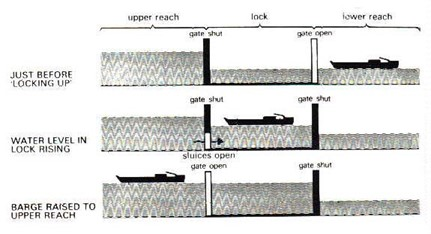
\includegraphics[scale=0.65]{sluismodel.jpg}

\subsubsection{Onderdelen}
Op basis van de schets kunnen we vaststellen dat een sluismodel uit de volgende onderdelen bestaat.

\begin{enumerate}
	\item Een tweetal sluisdeuren. 
	\item Een sluiskolk waarin de schepen in- enuitvaren
	\item een stoplicht om een signaal af te geven voor invaren en uitvaren.
	\item Een nivelleermachine zorgt ervoor dat het water in de sluis op het gewenste niveau wordt gebracht
	\item Een control-system dat ervoor zorgt dat de opdrachten van de sluisbeheerder (geautomatiseerd) worden uitgevoerd
\end{enumerate}
\subsubsection{Werking}

Een schip komt aanvaren en meld zich aan bij de sluismeester. De sluismeester geeft een signaal aan het controlsystem voor het openen van de sluisdeuren, nadat geccontroleerd is of de nivelleermachine al klaar is. Als er ruimte is voor een invarend schip mag het schip dat zoich heeft aangemeld en toestemming heeft  in de sluis varen. Op het moment dat de sluis vol is gaan de sluisdeuren dicht. Eenmaal afgesloten kan de nivelleermachine beginnen om het water in de sluiskolk op het gewenste waterpeil te brengen. Als dit nivelleerprces is afgerond geeft  het controlsystem daan da de sleusdeuren open kunnen.  Als de sleusdeuren open zijn en het uitvaarsignaal is op groen dan moet het schip in de sluis de sluis uitvaren.
\paragraph{extra cases}
Uit het zojuist genoemnde scenario valt het volgende op te maken.
\begin{enumerate}
	\item Een schip geeft een signaal aan een sluismeester.
	\item Er wordt gekeken of er wel plek is in de sluis .
	\item Er wordt gekeken of de nivelleermachine is afgerond.
	\item Er wordt gekeken wat het niveo van de waterpeil in de sluiskolk is.
	\item Er wordt gekeken of de sluisdeuren gereed zijn voor invarende schepen.
\end{enumerate}
\paragraph{Aandachtspunten}
\begin{enumerate}
	\item Voorrang tussen schepen onderling in de sluis?
	\item Hoe lang mag een schip zich in de sluis bevinden?
\end{enumerate} 

%%%%%%%%%%%%%%%%%%%%%%%%%%%%%%%%%%%%%%%%%%%%%%%%%%%%%%%%%%%%%%%%%
\section{Concept}

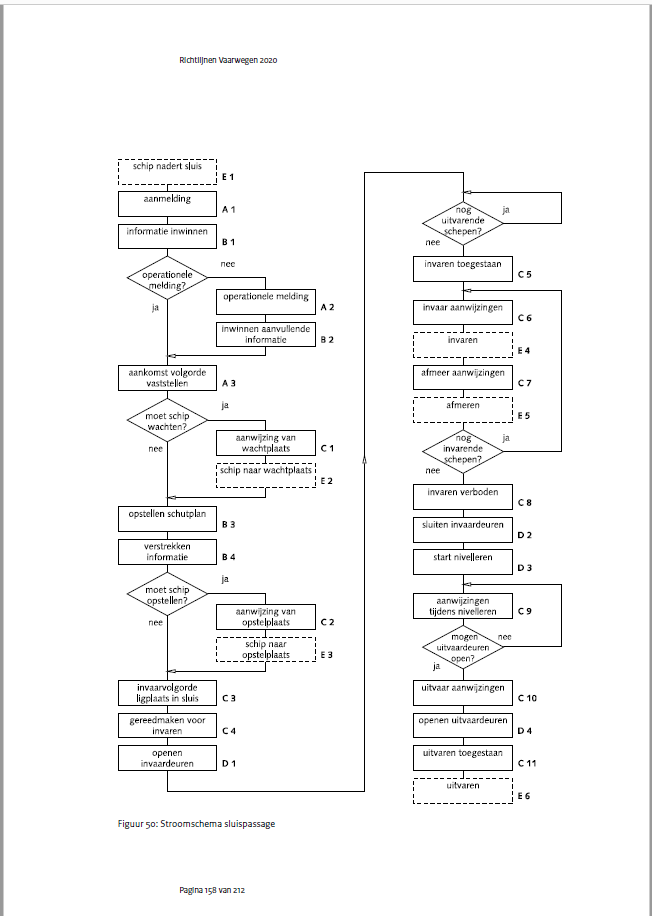
\includegraphics[scale=0.65]{sluispassage.png}

\paragraph{Vooraanmelding}


\paragraph{informatie inwinnen}


\paragraph{operationele melding}


\paragraph{aankomst volgorde}

\paragraph{aanwijzen wachtplaats}


\paragraph{verstrekken informatie}


\paragraph{aanwijzen opstelplaats}

\paragraph{opstellen schutproces}


\paragraph{verstrekken informatie}


\paragraph{invaarvolgorde en ligplaats in sluis}

\paragraph{gereedmaken voor invaren}



\paragraph{openen invaardeuren}




\paragraph{invaren toegestaan}

\paragraph{aanwijzingen voor invaren}
\paragraph{aanwijzingen tijdens afmeren}

\paragraph{invaren verboden}

\paragraph{sluiten invaardeuren}

\paragraph{start nivelleren}

\paragraph{aanzwijzingen voor uitvaren}
\paragraph{openen uitvaardewuren}

\paragraph{uitvaren toegestaan}




\paragraph{brainstorm 22-5-2022}

\subparagraph{invaardeuren en uitvaardeuren}
Gaan we uit van binnendeuren en buitendeuren? Er ontstaat dan een extra ruimte in de sluis. Hoeveel schepen kunnen in deze ruimte? Wat is de maximale wachtreij in deze ruimte en wat zijn de verkeersregels in deze nruimte?
\subparagraph{invaarstoplicht en uitvaarstoplicht}
Als invaren is toegestaan hoe wordt dit dan doorgegeven aan de schepen in de sluis? moeten zij dan uit zichzelf wachten of krijgen zij een signaal dat zij wewl/niet mogen uitvaren? En moeten zij dan kiezen voor links, midden of rechts? Of maakt dat allemaal niets uit?

\subparagraph{invaarwachtrij en uitvaarwachtrij}
Als er meerder schepen in een sluiskolk zitten moet het systeem dan rekeneing houden met het schip dat als eerste is ingevaren en/of het langst in de sluis zit?


%%%%%%%%%%%%%%%%%%%%%%%%%%%%%%%%%%%%%%%%%%%%%%%%%%%%%%%%%%%%%%%%%



\chapter{Kripke model}

\section{Uppaal kripke structuren}


\subsubsection{templates}

\paragraph{Schip}

\paragraph{Sluis}


\paragraph{Aanvoer}


\paragraph{Afvoer}

\paragraph{Pomp}

\paragraph{Pompbediening}


\paragraph{Stoplicht}

\paragraph{Deur}


\subparagraph{case}
Als een schip van rechts binnen komt en sluisdeuren zijn dicht dan moet het stoplicht op rood, de pomnp in transitie van laag naar hoog en niet andersom

\subparagraph{case}
Voor invaren geldt altijd: waterlevel, pomp uit, sluisdeuren open en stoplicht op groen

\subparagraph{case}
uitvarenden hebben voorang op invarenden

\subparagraph{case}
Voor invarenden geldt pomp uit, sleusdeur open en stoplicht op groen
\subparagraph{case}
voor nivelleren geldt pomp is aan, sluisduren zijn doicht en het stoplicht is op rood
\subparagraph{case}
Als een schip vertrekt dan zijn altijd, sleusdeuren open, waterlevel gereed op niveau 5 of 0 en stoplicht direct op groen
\subparagraph{case}
urgent locations; het is niet mogelijk om hier te wachten
\subparagraph{case}
urgent syn; een synchronisatie moet direct worden uitgevoerd als de guards geldig zijn

\subparagraph{case}
als een schip binnen is, en er zijn wachtende schepen, dan moet het stoplicht via oranje naar rood
\subparagraph{case}
committed; als deze staat actief is dan wordt de eerst volgende transitie uitaande van deze state
\subparagraph{case}
als een schjip binnen vaart mnoiet hij ook eft binnen zijn en niet binnenvaren, dit geldt ook voor sluisdeuren en pompen dus deze zijn committed.
\subparagraph{case}

\subparagraph{case}

\subparagraph{case}

\paragraph{Parallele compositie}


\paragraph{Parallele compositie}

\subsubsection{Modeleigenschappel}
\paragraph{Parallele compositie}
Om een sluispark te kunnen modelleren meerdere templates die de verschillende abstracties van het systeem aantonen.

\paragraph{Synchronisatgie}
Zorgt ervoor dat  een transitie die genomen worden in de ene kripke tructuur op hetzelfde moment wordt opgenomen in een andere kripke structuur.
\chapter{CTL logica}


\section{Doel van de test}
\subsection{Wat wordt getest en hoe}


\subsection{toetsen met queries}





\subsection{Operator: AG}
Voor alle paden


\subsection{Operator: EG}
Uiteindelijk geldt er een pad waarvoor geldt

\subsection{Operator: AF}
Voor alle paden/richtingen vroeg of laat
\subsection{Operator: EF}
Er is een pad
\subsection{Operator: AX}
Alle opvolgende toestanden

~\cite{locke_2020}
\subsection{Operator: EX}
Er bestaat vanaf de volgende minstens 1 state waarvoor geldt
\subsection{Operator: p U q}
Er geldt p tot q
~\cite{gnsguides}
\subsection{Operator: p R q}
q moet waar zijn totdat en inclusief de situatie dat p voor het eerst waar is, als p niet geldig is, dan moet q vooraltjd geldig zijn

\chapter{Testresultaten CTL logica}




\begin{center}
	\begin{tabular}{| l | c || r | }
		\hline
		1 &A[] !deadlock  &  TRUE \\ \hline
		2 & A[] not (Sluis.Tussenstop5 \&\& Deur.Klaar\_voor\_uitvaart)  &  Disconnected \\ \hline
		3 & A[]  (Sluis.Voorbereiden imply Deur.Dicht)   &  TRUE\\   \hline
		4 &A[]  (Deur.Dicht imply Counter==0)   & TRUE  \\   \hline
		5 & A[]  (Buitenstoplicht.Groen imply invaren\_allowed==true)  &  TRUE \\ \hline
		6 & A[] ! (Binnenstoplicht.Groen imply invaren\_allowed==false)  & FALSE \\ \hline
		7 & A[]  (globale\_tijd>30)   &  FALSE\\    \hline
		8 & E<>  (Schip.Stoppen and (Counter >5))   & Ship not a structure  \\   \hline
		9 & A[] (Schip.Vertrekken imply Sluisdeur.Dicht)  &  -  \\   \hline
		\hline
	\end{tabular}
\end{center}


 
%  https://www.stat.cmu.edu/~brian/latex/symbols/symbols.html
% https://tex.loria.fr/ctan-doc/macros/latex/doc/html/fntguide/node18.html
% https://observablehq.com/@s-haensch/latex-notation
% http://tdc-www.harvard.edu/tdcprop1/help/symbols/
% http://new.math.uiuc.edu/oldnew/netgeom/advice/to-texpad.html
% https://www.overleaf.com/learn/latex/List_of_Greek_letters_and_math_symbols
% https://jblevins.org/log/greek
% https://latex-tutorial.com/symbols/greek-alphabet/
% https://latex-programming.fandom.com/wiki/List_of_LaTeX_symbols
% https://physicsanduniverse.com/latex-symbols-and-using-them-to-write-equations/
% http://tug.ctan.org/info/symbols/comprehensive/symbols-a4.pdf
% https://tex.stackexchange.com/questions/99772/how-to-insert-greek-letters-having-trouble-with-greekletter
% https://texblog.org/2012/03/15/greek-letters-in-text-without-changing-to-math-mode/
% https://www.avantixlearning.ca/microsoft-word/how-to-insert-greek-letters-or-symbols-in-microsoft-word/
%
%
%








 
\paragraph{resultaat}


%	\bankstatement[title={Kontoauszug 12/2014},
%	openingbalance={-12,34},
%	closingbalance={82,13}]{201412.csv}
 
 
 
 
\subparagraph{verklareing}


\begin{filecontents*}{mydata.csv}
	1.8233,1.8233,1.8233,0.9243,0.8651,0.9013,0.3217,0.3377,34.4858
	0.2753,0.2753,0.2753,0.5383,0.5038,0.5249,0.3217,0.3377,8.4552
	0.0898,0.0898,0.0898,0.2804,0.2625,0.2734,0.3217,0.3377,1.5514
	0.4689,0.1193,0.0417,0.8046,0.2227,0.1795,0.6413,0.3307,6.4488
	0.339,0.8068,0.0936,0.4335,0.8036,0.2434,0.3046,0.624,20.8422
	0.2162,0.133,0.8711,0.1707,0.1503,0.8215,0.1562,0.0692,2.3365
	0.5187,0.9138,1.0432,0.4332,0.8028,0.8406,0.2269,0.3404,22.8164
	0.58,0.2096,0.9086,0.808,0.2134,0.8294,0.333,0.1596,8.4349
	0.8237,0.9378,0.0855,0.8654,0.8096,0.2487,0.4338,0.5187,26.9923 
\end{filecontents*}

\subsection{Fairness}
AG(AF(p))
\begin{verbatim}
	In welke staat de automaat zich ook bevindt, in alle richtingen kom je vroeg of laat een state tegen, waarin p geldig is.
\end{verbatim}
\subsection{Liveness}
\begin{verbatim}
	Altijd en overal geldt: Als p geldt dan geldt vroeg of laat q
	Ookal treedt p nooit p volgens de logica klopt het dan dat q volgt uit p.
	In een situatie, waarin p nooit optreedt, spreekt men van een
	vacuous truth.
\end{verbatim}

 
\VerbatimInput{mydata.csv}

\subsection{safety}
%\VerbatimInput{mydata.txt}

\subsection{zeno vrij}
Geen enkele state kan oneindig een transitie uitvoeren. Elke state heeft een uitgaande transitie.

\subsection{deadlocks}
%\VerbatimInput{data.txt}
 





